%%%%%%%%%%%%%%%%%%%%%%%%%%%%%%%%%%%%%%%%%%%%%%%%%%%%%%%%%%%%%%%%%%%%%%
% How to use writeLaTeX: 
%
% You edit the source code here on the left, and the preview on the
% right shows you the result within a few seconds.
%
% Bookmark this page and share the URL with your co-authors. They can
% edit at the same time!
%
% You can upload figures, bibliographies, custom classes and
% styles using the files menu.
%
%%%%%%%%%%%%%%%%%%%%%%%%%%%%%%%%%%%%%%%%%%%%%%%%%%%%%%%%%%%%%%%%%%%%%%

\documentclass[12pt]{article}

\usepackage{sbc-template}

\usepackage{graphicx,url}

%\usepackage[brazil]{babel}   
\usepackage[utf8]{inputenc}  

\usepackage{code}

\usepackage{amsmath}
     
\sloppy

\title{Implementação e Análise de Matrizes Esparsas Utilizando Listas Encadeadas Circulares}

\author{Antonio Willian Silva Oliveira\inst{1}, Iago de Oliveira Lo\inst{2}}


\address{Aluno do Campus Quixadá (CE)– Universidade Federal do Ceará (UFC) 
 \\ Av. José de Freitas Queiroz, 5003 – Cedro – Quixadá – Ceará 63902-580– Brazil \\
\nextinstitute
 Aluno do Campus Quixadá (CE)– Universidade Federal do Ceará (UFC) \\
Av. José de Freitas Queiroz, 5003 – Cedro – Quixadá – Ceará 63902-580– Brazil 
  \email{williansilva@alu.ufc.br, iagooliveiralo07@alu.ufc.br}
}

\begin{document} 

\maketitle

\begin{abstract}
  The adopted structure uses circular linked lists to represent the rows and columns of the matrix, allowing dynamic and efficient access to nonzero elements. Each node points to the next in the same row and to another in the same column, which is in the next row, ensuring the circularity of the matrix. This method prevents memory waste and improves performance compared to conventional matrices.
During development, we faced challenges such as maintaining the circularity of the linked lists and managing memory. The tests performed indicated that the implemented structure correctly performs its function as expected and is efficient for large sparse matrices, significantly reducing memory usage.
We conclude that using circular linked lists to represent sparse matrices is a viable and advantageous approach, especially for applications that require high efficiency.
\end{abstract}
     
\begin{resumo} 
  Neste relatório, apresentamos a implementação de uma matriz esparsa circular utilizando listas encadeadas. O objetivo foi desenvolver uma estrutura eficiente para armazenar e manipular matrizes esparsas, economizando espaço e facilitando operações como inserção, soma e multiplicação.
A estrutura adotada utiliza listas encadeadas circulares para representar as linhas e colunas da matriz, permitindo um acesso dinâmico e eficiente aos elementos não nulos. Cada nó aponta para o próximo na mesma linha e para outro da mesma coluna, que está na linha seguinte, garantindo a circularidade da matriz. Esse método evita desperdício de memória e melhora o desempenho em comparação com matrizes convencionais.
Durante o desenvolvimento, enfrentamos desafios como a manutenção da circularidade das listas encadeadas e o gerenciamento da memória. Os testes realizados indicaram que a estrutura implementada executa corretamente sua função conforme o esperado e é eficiente para matrizes esparsas grandes, reduzindo significativamente o uso de memória.
Concluímos que o uso de listas encadeadas circulares para representar matrizes esparsas é uma abordagem viável e vantajosa, especialmente para aplicações que demandam alta eficiência.
\end{resumo}


\section{Introdução} 

As matrizes se caracterizam como arranjos bidimensionais de números organizados em linhas e colunas, sendo bastante utilizadas, por exemplo, nas áreas de matemática, computação e programação. Nesse contexto, é importante evidenciar que o uso de matrizes na computação e na programação enfrenta um grande desafio: quanto maior o número de elementos de uma matriz, maior será a quantidade de dados armazenados na memória. Por isso, uma forma de tentar minimizar os danos causados por esse problema é o uso da Sparse Matrix.

A Sparse Matrix (Matriz Esparsa) é uma matriz que possui como característica o grande número de elementos nulos ou iguais a 0. Por causa disso, seu uso busca armazenar na memória apenas valores não nulos ou diferentes de 0, fazendo com que a quantidade de dados armazenados diminua consideravelmente. Essa característica a torna especialmente útil quando a eficiência de armazenamento e o desempenho computacional são essenciais na aplicação. 

Este trabalho tem como objetivo apresentar a Matriz Esparsa, mostrando detalhes da sua implementação e da sua aplicação.

\section{Estrutura de Dados Implementada} \label{sec:EstruturadeDadosImplementada}
A implementação da matriz esparsa baseia-se em uma abordagem dinâmica e modular, que utiliza exclusivamente a alocação de memória por nós, em vez do uso tradicional de arrays. Essa estratégia permite representar eficientemente matrizes em que a grande maioria dos elementos é nulo. A matriz esparsa utiliza uma estrutura de dados flexível e escalável que proporciona uma alocação de memória otimizada, evitando desperdícios significativos e promovendo maior eficiência no armazenamento e processamento.

    \subsection{Representação dos Nós}
    Cada elemento relevante da matriz é encapsulado em um nó, definido pela estrutura Node. Esse nó contém os seguintes campos:
    
\begin{lstlisting}[caption={Estrutura do Nó em C++}]
    struct Node {
        Node *direita;  // (direcao horizontal)
        Node *abaixo;   // (direcao vertical)
        int linha;
        int coluna;
        double valor;
    };
\end{lstlisting}

\begin{itemize}
    \item \textbf{Valor:} Representa o dado numérico armazenado na célula.
    \item \textbf{Índices (linha e coluna):} Indicam a posição do elemento dentro da matriz.
    \item  \textbf{Ponteiros direita e abaixo:} Estes ponteiros conectam o nó aos seus vizinhos na mesma linha e coluna, respectivamente.
\end{itemize}

\subsection{Estrutura da Matriz}

\begin{figure}[ht]
    \centering
    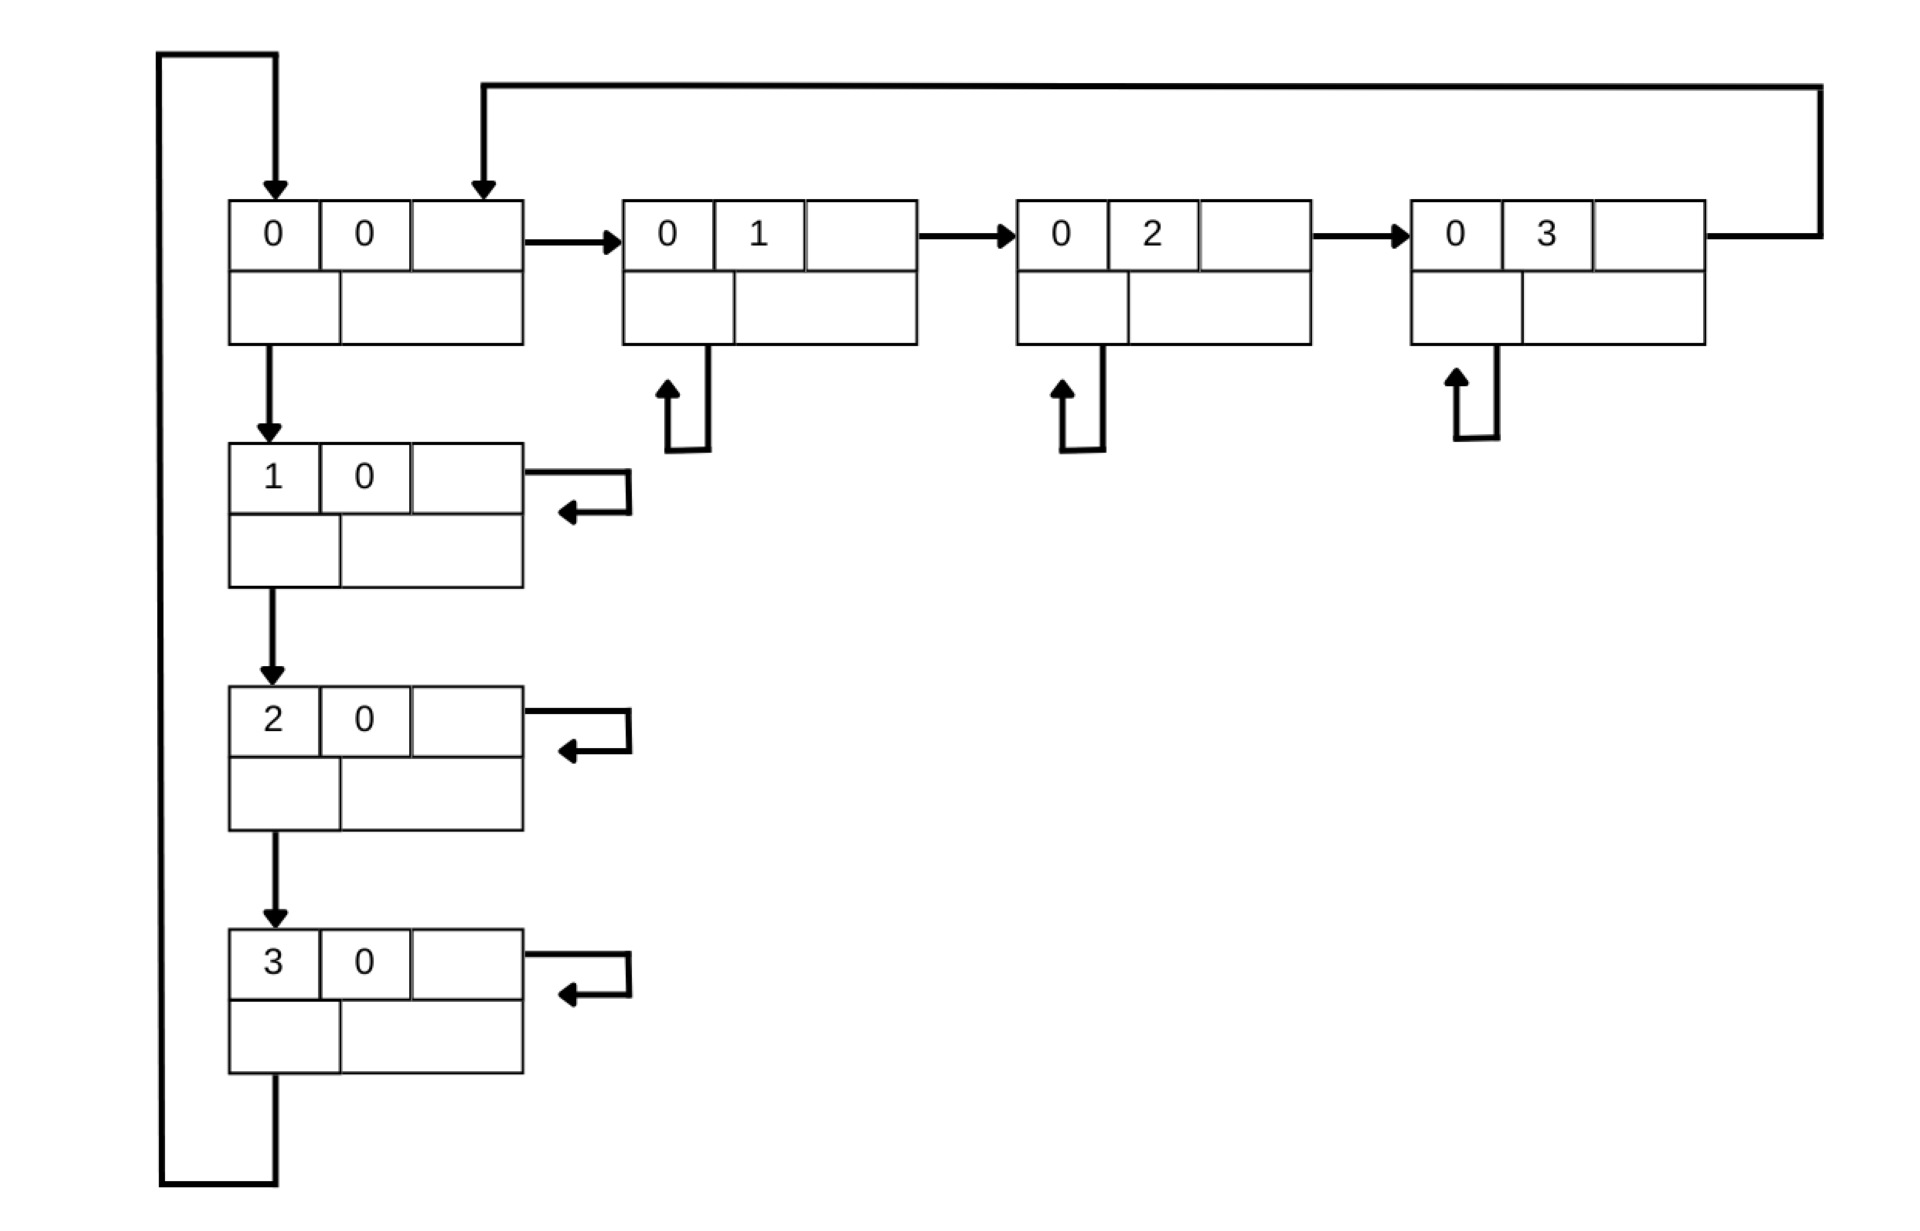
\includegraphics[width=.8\textwidth]{matrixVazia.png}
    \caption{Esquema de uma Matriz Esparsa vazia.}
    \label{fig:Esquema de uma Matriz Esparsa vazia}
\end{figure}

A classe Matriz utiliza um nó especial denominado cabeçalho (ou "sentinela"), que serve como ponto de referência para toda a estrutura. A partir deste nó, são geradas duas listas circulares:

\begin{itemize}
    \item \textbf{Lista de Linhas:} Cada linha da matriz é representada por uma lista circular de nós. Durante a construção, para cada linha, um novo nó sentinela é criado e ligado através do ponteiro abaixo. Ao final do laço, a última linha aponta de volta para o nó cabeçalho, completando a circularidade vertical da estrutura.
    
    \item \textbf{Lista de Colunas:} Similarmente, cada coluna é organizada como uma lista circular. Os nós sentinelas para as colunas são gerados e conectados através do ponteiro direita, e a última coluna retorna ao cabeçalho, estabelecendo a circularidade horizontal.
\end{itemize}

\subsection{Iterador para a Matriz}
A classe IteratorM permite percorrer a matriz de forma sequencial, abstraindo os detalhes de navegação das listas circulares. O iterador é definido com os seguintes atributos:

\begin{lstlisting}[caption={Estrutura do Iterator em C++}]
    class IteratorM {
        Node *cabecalho;
        Node *current;
}
\end{lstlisting}

\begin{itemize}
    \item \textbf{Ponteiro para o nó cabeçalho:} Permite manter o ponto de referência da estrutura.
    \item \textbf{Ponteiro para o nó atual}: Indica a posição corrente durante a iteração.
    \item Os operadores sobrecarregados (como \textbf{\textit{operator*}}, \textbf{\textit{operator\(\xrightarrow{}\)}} e \textbf{\textit{operator++}}) possibilitam a utilização de construções típicas de iteração (por exemplo, em laços for) para acessar os valores dos nós, garantindo uma interface consistente e intuitiva para o usuário da estrutura.
\end{itemize}

\section{Decisões de Implementação}
Durante o desenvolvimento deste projeto, as decisões sobre a implantação foram tomadas após uma análise dos requisitos, considerando as limitações impostas pelo problema específico e as diversas abordagens possíveis. Para cada uma dessas abordagens, avaliamos aspectos como complexidade computacional, facilidade de manutenção e impacto na performance. O foco principal dessas escolhas foi otimizar fatores essenciais, como a eficiência do sistema, a escalabilidade para suportar crescimento futuro e a robustez da solução em relação a possíveis falhas ou imprevistos. Além disso, buscamos garantir que a implementação atendesse de forma eficaz e equilibrada tanto aos objetivos de desempenho quanto às limitações de uso de memória, visando proporcionar uma solução que fosse não apenas funcional, mas também sustentável e capaz de se adaptar a diferentes cenários de utilização.

    \subsection{Abstração através de Iteradores}
        Uma de nossas decisões foi criar um iterador personalizado, chamado \textbf{IteratorM}, com o intuito de isolar a complexidade associada à navegação na estrutura de dados. Essa decisão visou estabelecer uma interface de iteração que abstraísse completamente os detalhes internos da organização dos nós, permitindo que os usuários da matriz percorressem os elementos não nulos de forma sequencial e intuitiva, sem a necessidade de compreender a implementação subjacente. O iterador foi desenvolvido para suportar operações fundamentais, como desreferenciação e incremento, seguindo os princípios e paradigmas da biblioteca padrão do C++, garantindo compatibilidade e consistência com as práticas comuns da linguagem.

        Além de proporcionar uma navegação eficiente e transparente, essa abstração facilita o uso da estrutura de dados e contribui para a modularização do código. Com a separação das responsabilidades de iteração, o código torna-se mais coeso e de fácil manutenção, pois alterações na implementação interna da estrutura de dados não afetam diretamente a forma como os usuários interagem com ela. Assim, a implementação do \textbf{IteratorM} assegura uma solução que é, ao mesmo tempo, flexível, escalável e de fácil adaptação a futuras modificações ou expansões.

\section{Divisão do Trabalho}
O desenvolvimento deste projeto foi realizado em colaboração, com responsabilidades distribuídas de maneira estratégica após algumas sessões de brainstorming, garantindo uma integração eficaz entre as diferentes fases da implementação. A seguir, detalhamos como o trabalho foi organizado e as principais responsabilidades atribuídas a cada membro da equipe.

    \subsubsection{Responsabilidades Individuais e Colaborativas}
    \begin{itemize}
        \item \textbf{Responsável:} Willian Silva
            \begin{itemize}
                \item Desenvolvimento e Implementação da Interface Visual do Programa (Função Principal - Main);
                \item Desenvolvimento dos métodos de construção e de soma entre matrizes;
                \item Criação e integração dos nós sentinelas para a formação das listas circulares, assegurando a conexão entre linhas e colunas.
            \end{itemize}

        \item \textbf{Responsável:} Iago de Oliveira:
            \begin{itemize}
                \item Desenvolvimento das funções de acesso (get), limpeza, liberação de memória e operação de multiplicação de matrizes, com foco na eficiência e na correta manipulação dos nós;
                \item Realização de testes unitários e de integração para validar a funcionalidade de cada operação, assegurando a aderência aos requisitos de desempenho e integridade estrutural;
                \item Implementação da classe iteradora (IteratorM), que permite a navegação sequencial e a abstração dos detalhes internos da estrutura de dados.
            \end{itemize}

        \item \textbf{Responsabilidade Compartilhada}
            \begin{itemize}
                \item  Implementação do método de Inserção (Insert);
                \item Elaboração do relatório técnico, documentando detalhadamente a estrutura de dados implementada, as decisões de implantação, as dificuldades encontradas e os resultados dos testes;
                \item Realização da análise de complexidade das funções críticas (insert, get e sum), com a descrição dos casos de pior cenário e justificativas teóricas para os resultados obtidos;
                \item Compilação dos resultados dos testes e validação do comportamento da matriz esparsa em cenários variados, garantindo que a solução fosse robusta e escalável.
                \item Revisão final do código e da documentação, assegurando a coerência e a clareza de todo o material entregue;
                \item Identificação e correção de bugs, além da otimização dos algoritmos de busca e inserção.
            \end{itemize}
    \end{itemize}

\section{Dificuldades Encontradas}
Durante o desenvolvimento deste projeto, identificamos e enfrentamos diversos desafios técnicos e conceituais. Esses obstáculos exigiram uma análise aprofundada e soluções criativas para garantir a integridade e a eficiência da implementação. A seguir, apresentamos as principais dificuldades encontradas e as estratégias adotadas para superá-las:
    \subsubsection{Manutenção da Circularidade das Listas Encadeadas}
        Uma das maiores dificuldades iniciais foi criar listas encadeadas circulares para representar as linhas e colunas. Garantir que o nó cabeçalho estivesse corretamente conectado a ambas as listas (horizontal e vertical) foi essencial para preservar a integridade da estrutura. Durante a fase de testes, constatou-se que pequenas inconsistências na lógica de fechamento das listas poderiam resultar em loops infinitos ou falhas na navegação, comprometendo a execução das operações de inserção, busca e iteração. A resolução desse problema exigiu uma revisão minuciosa dos algoritmos de conexão e a implementação de condições de parada bem definidas, além de uma série de testes rigorosos para validar a consistência da circularidade em diversos cenários.
    \subsubsection{Gerenciamento de Memória Dinâmica}
        Outra dificuldade bastante significativa foi o gerenciamento eficiente da memória, pois toda a estrutura da matriz esparsa depende exclusivamente da alocação dinâmica de nós. A ausência de arrays ou estruturas fixas fez com que cada inserção e remoção demandasse atenção especial para evitar vazamentos de memória. Para mitigar esse risco, foi necessário desenvolver mecanismos robustos de limpeza e liberação de recursos, como a função limpar(), que percorre de forma segura e sistemática toda a estrutura. A implementação exigiu rigor na verificação das conexões entre nós e na manutenção da circularidade, garantindo que nenhum nó permanecesse alocado inadvertidamente após a finalização das operações.
    \subsubsection{Implementação e Integração do Iterador}
    A criação da classe iteradora (IteratorM) foi um ponto crítico para facilitar a navegação na estrutura. O iterador precisava abstrair a complexidade interna da matriz esparsa, permitindo que o usuário percorresse os elementos não nulos de forma intuitiva. No entanto, a implementação do operador de incremento apresentou desafios, especialmente em relação à manutenção da circularidade da estrutura, evitando que o iterador entrasse em um loop infinito. Além disso, a necessidade de manter a coerência entre o nó atual e o cabeçalho exigiu uma série de ajustes finos e a implementação de condições de verificação, além de testes para garantir que a interface do iterador fosse robusta e confiável.

Em síntese, as dificuldades enfrentadas durante o desenvolvimento do projeto foram superadas por meio da combinação de análise teórica, desenvolvimento iterativo e rigorosos testes de validação. Esses desafios não apenas contribuíram para o aprimoramento da solução, mas também proporcionaram um aprendizado valioso sobre técnicas avançadas de gerenciamento de memória, manutenção de estruturas circulares e otimização de algoritmos, consolidando a base para futuras implementações.
    
\section{Testes Executados}

    A criação de um arquivo responsável pela execução de teste foi necessário para validar as operações fundametais da Matriz Esparsa, tais como inserção de valores, soma, multiplicação e análise de desempenho. Dessa forma, os testes buscam garantir a corretude e a eficiência das operações implementadas na matriz.

    \subsection{Metodologia}
    Os testes foram implementados em C++ e utilizam as bibliotecas iostream, fstream, stdexcept e chrono. As funções principais testadas são:
    
    \subsubsection{Teste de Inserção}

    Neste teste, uma matriz 5x5 é inicialmente criada com todos os seus elementos definidos como nulos. Em seguida, utiliza-se a função insert() para inserir valores em posições específicas da matriz. Por exemplo, podem ser inseridos:

    \begin{itemize}
        \item  O valor 1 na posição (1, 1);
        \item  O valor 2 na posição (5, 5);
        \item  O valor 2 na posição (3, 2).
    \end{itemize}
    
    Após cada inserção, a função get() é utilizada para recuperar o valor armazenado na posição correspondente. A verificação é feita utilizando o assert(), que compara o valor retornado com o valor esperado. Caso haja divergência, o assert() dispara um erro, indicando que a operação de inserção não foi realizada corretamente.
    
    Esta abordagem garante que cada inserção seja validada individualmente, facilitando a identificação de possíveis problemas na implementação da função insert().

   \subsubsection{Teste de Soma de Matrizes com mesmo número de linhas e colunas(tamanho)}

    Neste teste, três matrizes são carregadas a partir de arquivos externos. Duas delas representam os operandos que serão somados utilizando a função \texttt{sum()}, enquanto a terceira contém o resultado esperado para essa operação.
    
    Após a execução da função \texttt{sum()}, o teste procede à verificação dos resultados. Para isso, é utilizado o método \texttt{get()} para acessar cada elemento da matriz resultante e da matriz esperada, comparando os valores correspondentes. Se for detectada qualquer discrepância entre os valores, uma exceção é lançada, indicando que houve falha na implementação da soma.
    
    Esta abordagem garante que tanto as dimensões quanto os valores individuais das matrizes sejam validados, assegurando a correção da operação de soma.
    
    
     \subsubsection{Teste de Multiplicação de Matrizes com mesmo tamanho}
    
    Similar ao teste de soma, mas utilizando a função \texttt{multiply()}. Três matrizes são carregadas a partir de arquivos, sendo duas as matrizes que serão multiplicadas e a terceira como o resultado do produto.

    Após a multiplicação, o método \texttt{get()} é chamado para acessar cada elemento da matriz resultante e da matriz esperada, comparando os valores correspondentes. Se for detectada qualquer discrepância entre os valores, uma exceção é lançada, indicando que houve falha na implementação da multiplicação.

    \subsubsection{Teste de Multiplicação e de Soma com Matrizes de Tamanhos Diferentes}

    Neste teste, avaliamos o comportamento das funções \texttt{sum()} e \texttt{multiply()} quando aplicadas a matrizes com dimensões incompatíveis para as operações pretendidas.
    
    Para a soma, a regra é que ambas as matrizes devem possuir o mesmo número de linhas e colunas. Já para a multiplicação, é necessário que o número de colunas da primeira matriz seja igual ao número de linhas da segunda. No cenário testado, as matrizes utilizadas não atendem a nenhum desses critérios, ou seja, suas dimensões são incompatíveis para realizar a soma ou a multiplicação.
    
    Para garantir um tratamento adequado dos erros, as chamadas às funções \texttt{sum()} e \texttt{multiply()} foram encapsuladas em blocos \texttt{try { }} \texttt{catch(\ldots)}, de forma que quaisquer exceções lançadas devido às incompatibilidades de tamanho sejam capturadas e processadas. O comportamento esperado é que, ao tentar realizar as operações, a aplicação lance exceções informando claramente o problema de dimensão, e assim, o programa se comporta de forma robusta ao detectar e tratar entradas inválidas.
    
    Esta abordagem confirma que o sistema é capaz de identificar e reportar erros quando as operações são solicitadas com matrizes de tamanhos diferentes, evitando resultados inesperados e garantindo a integridade da aplicação.
    
    \subsubsection{Teste de Performance}

    O objetivo deste teste é medir o tempo de execução, em milissegundos (ms), das funções \texttt{sum()} e \texttt{multiply()} utilizadas na manipulação de matrizes esparsas.
    
    Para a realização do teste, são criadas duas matrizes de dimensão 100x100. A primeira matriz é preenchida com valores definidos pelo padrão i + j, onde i representa o índice da linha e j o índice da coluna. A segunda matriz, por sua vez, é preenchida utilizando o padrão i - j.
    
    A medição do tempo é realizada com o auxílio da biblioteca \texttt{chrono}. São registrados os instantes de início e término da execução das operações, permitindo o cálculo da duração de cada função em milissegundos. Ao final, os tempos obtidos são exibidos no console, fornecendo uma avaliação da performance das funções \texttt{sum()} e \texttt{multiply()}.
    
\section{Análise de Complexidade}
    \subsection{Função \texttt{Insert()}}

    A função \texttt{insert()} é uma das operações centrais na implementação da matriz esparsa, responsável por inserir novos elementos (não nulos) na estrutura de dados que representa a matriz. 
    
    Por isso, a análise de complexidade dessa função nos permite identificar os pontos críticos e determinar o pior caso teórico da operação. Nesta análise, serão considerados os passos envolvidos na busca da posição correta para inserção—tanto na dimensão das linhas quanto das colunas—e os ajustes dos ponteiros na estrutura de dados. 
    
    Além disso, é importante observar que a função insert() primeiramente verifica se existe valor na posição desejada e, caso exista, atualiza o valor. No entanto, caso não exista, é feita a criação de um novo nó.

    \subsubsection{Verificação inicial:}
        \begin{itemize}
            \item A comparação if (value == 0) e a validação dos índices (\textbf{if} (posI \(\leq\) 0 \(||\) posI \(>\) linhas \(||\) posJ \(\leq\) 0 \(||\) posJ \(>\) colunas)) são operações em tempo constante, ou seja, O(1).
    
            \item Busca na Lista Horizontal (Percorrendo Linhas) para encontrar a posição desejada:
            \begin{lstlisting}
                Node *linhaAtual = cabecalho;
                while (linhaAtual->linha < posI)
                {
                    linhaAtual = linhaAtual->abaixo;
                }
        
            \end{lstlisting}
            \item Nesse loop, começamos a partir do nó cabeçalho e vamos descendo pela lista vertical até atingir a linha posI. 
            
            \item No pior caso, se posI for a última linha, o loop executará linhas iterações, tendo, assim, complexidade O(linhas). 
        \end{itemize}
    
    \subsubsection{Busca na Lista Vertical (Percorrendo Colunas). Loop para encontrar a coluna desejada:}
        \begin{lstlisting}
            Node *colunaAtual = cabecalho;
            while (colunaAtual->coluna < posJ)
            {
                colunaAtual = colunaAtual->direita;
            }
        
        \end{lstlisting}
        \begin{itemize}
                \item Aqui, percorremos os nós na lista horizontal para alcançar a coluna posJ. 
                
                \item No pior caso, se posJ for a última coluna, o loop executará colunas iterações. Complexidade: O(colunas).
        \end{itemize}

    \subsubsection{Busca na Lista Horizontal para a criação do novo nó:}
        \begin{lstlisting}
            Node *aux = linhaAtual;
            while (aux->direita != linhaAtual && aux->direita->coluna < posJ)
            {
                aux = aux->direita;
            }
        \end{lstlisting}
        \begin{itemize}
            \item Caso não haja valor na posição indicada, esse loop percorre os nós na linha para localizar a posição onde o novo nó deve ser inserido. 
            
            \item No pior caso, se a linha estiver muito “cheia” (ou seja, se houver muitos nós não nulos nessa linha), o número de iterações pode ser proporcional ao número de elementos na linha. Em uma matriz densamente preenchida, isso poderia se aproximar de O(colunas).
        \end{itemize}

    \subsubsection{Busca na Lista Vertical para a criação do novo nó:}
        \begin{lstlisting}
            aux = colunaAtual;
            while (aux->abaixo != colunaAtual && aux->abaixo->linha < posI)
            {
                aux = aux->abaixo;
            }
    
        \end{lstlisting}
        \begin{itemize}
            \item Esse loop percorre os nós na coluna para inserir o novo nó na posição adequada.
    
            \item No pior caso, se a coluna tiver muitos nós, o número de iterações pode ser proporcional ao número de elementos nessa coluna (até O(linhas) no pior cenário).
        \end{itemize}

    \subsubsection{Inserção do Novo Nó:}
        \begin{itemize}
            \item As operações de ajuste dos ponteiros para inserir o novo nó na lista horizontal e vertical são operações em tempo constante \(O(1)\).
        \end{itemize}

    \subsubsection{Conclusão}
    Portanto, a complexidade total da função insert() é da ordem de O(linhas + colunas) no pior cenário, onde cada dimensão é percorrida independentemente.
    
    \subsection{Função \texttt{Get()}}

    A função \texttt{get()} tem a finalidade de recuperar o valor de um elemento armazenado na matriz esparsa. Como essa estrutura armazena apenas os elementos não nulos em uma lista encadeada bidimensional (organizada em linhas e colunas), a busca por um elemento específico deve percorrer os nós existentes até encontrar a posição desejada.  
    
    Para realizar essa busca, a função utiliza um iterador \texttt{IteratorM}, que percorre os elementos da matriz de forma ordenada. A estratégia de busca adotada avança pelo iterador enquanto o nó atual estiver "antes" da posição desejada, garantindo que o acesso seja realizado de maneira eficiente.  

        \subsubsection{A implementação da função \texttt{get()} segue os seguintes passos principais:} 
    
            \begin{itemize} 
                \item  \textbf{Validação dos Índices} \\ 
                   Antes de realizar a busca, a função verifica se os índices informados (\texttt{posI}, \texttt{posJ}) são válidos. Caso contrário, uma exceção é lançada. Essa verificação ocorre em \(O(1)\).  
                
                \item \textbf{Inicialização do Iterador} \\
                   A busca é realizada por meio do iterador \texttt{IteratorM}, que percorre os elementos da matriz esparsa começando do primeiro elemento armazenado.  
                
                \item \textbf{Busca Sequencial pelo Elemento} \\
                   O loop principal da função percorre os nós armazenados até encontrar a posição desejada ou até ultrapassá-la. Esse processo ocorre no trecho:  
        
            \begin{lstlisting}
    while (it != end() && (it.current->linha < posI || (it.current->linha == posI && it.current->coluna < posJ)))
        {
            ++it;
        }
        
            \end{lstlisting}
               
               Esse trecho percorre os nós existentes de maneira ordenada, avançando até encontrar a posição desejada.  
            
            \item \textbf{Verificação e Retorno do Valor} \\
               - Se o nó encontrado corresponder exatamente à posição (\texttt{posI}, \texttt{posJ}), a função retorna seu valor.  \\
               - Caso contrário, a função retorna 0, indicando que a posição não está armazenada na matriz esparsa.  
            
            \end{itemize}

        \subsubsection{Análise de Complexidade:}
        
        A eficiência da função \texttt{get()} depende do número de elementos armazenados na matriz e da posição do elemento buscado. 
    
            \begin{itemize}
                \item \textbf{Melhor Caso – \(O(1)\)}
                Se a matriz for muito esparsa e a posição buscada não estiver armazenada, a função pode rapidamente identificar a ausência do elemento e retornar 0 sem percorrer toda a estrutura. Isso acontece quando a busca para logo no início, tornando a complexidade \(O(1)\). 
                
                \item \textbf{Caso Médio – \(O(k)\)}, onde \(k\) é o número de elementos não nulos percorridos 
                Em uma matriz esparsa comum, a busca precisa percorrer apenas os nós armazenados, ou seja, os elementos não nulos. O tempo de execução dependerá do número de elementos existentes antes da posição desejada. Dessa forma, esse valor será pequeno, tornando a busca eficiente. 
                
                \item \textbf{Pior Caso – \(O(n)\)}, onde n é o número total de elementos não nulos
                No pior cenário, se a matriz estiver quase cheia (com poucos elementos nulos), a busca pode precisar percorrer todos os elementos antes de encontrar a posição desejada. Nesse caso, a complexidade pode chegar a \(O(n)\), onde \(n\) é o número total de elementos não nulos da matriz.  
                
                No entanto, mesmo nesse cenário, o desempenho ainda pode ser melhor que uma busca em uma matriz densa tradicional, pois a função só percorre elementos realmente armazenados.  
                
            \end{itemize} 
    
        \subsubsection{Conclusão:}
        
        A complexidade da função \texttt{get()} varia conforme a estrutura da matriz:  

        \begin{itemize}
            \item  \textbf{\(O(1)\)} no melhor caso (quando o elemento não existe e é rapidamente identificado).
            \item  \textbf{\(O(k)\)} no caso médio (onde k é o número de elementos não nulos percorridos). 
            \item  \textbf{\(O(n)\)} no pior caso (quando precisa percorrer todos os elementos armazenados).  
        \end{itemize}
        
        Em uma matriz esparsa típica, a complexidade esperada tende a ser \textbf{\(O(k)\)}, tornando a busca eficiente. Dessa forma, a estrutura da matriz esparsa permite um acesso relativamente rápido aos elementos armazenados, mesmo sem o uso de uma indexação tradicional.  
    
    \subsection{Função \texttt{Sum()}}
        A função \texttt{sum} tem o objetivo de somar duas matrizes (digamos, matrixA e matrizB) e retornar uma nova matriz com o resultado da soma. A estrutura do código é a seguinte:
        
            \subsubsection{Verificação das Dimensões}
                \begin{lstlisting}
    if (matrixA.getLinhas() != matrizB.getLinhas() || matrixA.getColunas() != matrizB.getColunas())
    {
        throw std::invalid_argument("Erro: As matrizes nao possuem o mesmo tamanho");
    }
                \end{lstlisting}
            Nesta etapa, são feitas duas comparações simples para verificar se o número de linhas e colunas das matrizes matrixA e matrizB são iguais. Comparar valores inteiros é uma operação de tempo constante.

            \begin{itemize}
                \item Complexidade desta etapa: \(O(1)\)
            \end{itemize}

Esta etapa é extremamente eficiente e não influencia significativamente na complexidade total da função.

    \subsubsection{Criação da Nova Matriz}
    \begin{lstlisting}
Matriz matriz(matrixA.getLinhas(), matrixA.getColunas());
    \end{lstlisting}
A criação da nova matriz é feita através do construtor da classe Matriz. O construtor é responsável por inicializar os cabeçalhos de linha e coluna, criando uma estrutura que facilita o acesso e a inserção de elementos.
    \begin{itemize}
        \item O que o Construtor Faz:
            \begin{itemize}
                \item Inicializa o cabeçalho principal com um nó que aponta para si mesmo.
                \item Cria nós cabeçalho para cada linha: Um laço de 1 até n (onde n é o número de linhas) cria um nó para cada linha.
                \item Cria nós cabeçalho para cada coluna: Outro laço de 1 até m (onde m é o número de colunas) cria um nó para cada coluna.
            \end{itemize}

        \item Complexidade da Criação da Matriz:
             Como cada linha e coluna é inicializada separadamente a complexidade será \(O(n + m)\), sendo \(n\) o número de linhas e \(m\) o número de colunas

        
    \end{itemize}
            Esta etapa é linear em relação à soma das dimensões da matriz, o que é eficiente considerando o contexto geral.

    \subsubsection{Iteração Sobre os Elementos}
\begin{lstlisting}
    for (int i = 1, linha = matrixA.getLinhas(); i <= linha; i++)
{
    for (int j = 1, coluna = matrixA.getColunas(); j <= coluna; j++)
    {
        double valor = matrixA.get(i, j) + matrizB.get(i, j);
        matriz.insert(i, j, valor);
    }
}
\end{lstlisting}

A função utiliza dois laços aninhados para percorrer todos os elementos da matriz. O laço externo percorre as linhas e o laço interno percorre as colunas.

    \begin{itemize}
        \item \textbf{Número total de iterações}: \(n \cdot m\)
            \begin{itemize}
                \item Onde \(n\) é o número de linhas e \(m\) o número de colunas.
            \end{itemize}

            \item Cada iteração realiza duas operações principais:
                \begin{itemize}
                    \item Acesso aos valores com o método get.
                    \item Inserção do valor somado com o método insert.
                \end{itemize}
    \end{itemize}
A seguir, detalharemos a complexidade dessas operações.

    \subsubsection{Acesso aos Valores com o Método \texttt{get}}
\begin{lstlisting}
    double valor = matrixA.get(i, j) + matrizB.get(i, j);
\end{lstlisting}

O método \texttt{get} é responsável por acessar o valor na posição (i, j) da matriz. A busca é feita percorrendo a lista ligada até encontrar o nó correspondente.

\begin{itemize}
    \item Como o \texttt{get} Funciona:
        \begin{itemize}
            \item Começa no nó cabeçalho da matriz.
            \item Percorre a lista até encontrar a linha i.
            \item Dentro da linha i, percorre até encontrar a coluna j.
        \end{itemize}
\end{itemize}

\textbf{Complexidade do \texttt{get}:} 
    O pior caso ocorre quando o elemento desejado está no final da linha ou coluna, o que exige percorrer todos os nós daquela linha ou coluna.

    \begin{itemize}
        \item \textbf{Complexidade por chamada:} 
        \begin{equation}
            O(max(n, m)
        \end{equation}
    \end{itemize}

Como cada iteração da função \texttt{sum} faz duas chamadas ao \texttt{get} (uma para cada matriz), o custo total por iteração é:

\begin{itemize}
    \item \textbf{Complexidade total do get por iteração:} 
        \begin{equation}
            2 \cdot O(max(n, m) = O(max(n, m)
        \end{equation}
\end{itemize}

\subsubsection{Inserção com o Método \texttt{insert}}

\begin{lstlisting}
    matriz.insert(i, j, valor);
\end{lstlisting}

O método insert insere um novo valor na posição (i, j) da matriz, considerando a estrutura esparsa.

\begin{itemize}
    \item Como o insert Funciona:
        \begin{itemize}
            \item Verifica se o valor é zero. Se for, não insere.
            \item Percorre a lista de nós na linha i até encontrar a posição correta.
            \item Se o nó já existir, atualiza o valor; caso contrário, cria um novo nó.
            \item Repete o processo para a coluna j para manter a estrutura consistente.
        \end{itemize}

    \item Complexidade do \texttt{insert}: 
        \begin{equation}
            O(n + m)
        \end{equation}
\end{itemize}

\subsubsection{Complexidade Total da Função \texttt{sum}}

Agora, combinamos as complexidades das etapas:

    \begin{enumerate}
        \item Verificação das dimensões: \(O(1)\)
        \item Criação da nova matriz: \(O(n + m)\)
        \item Iteração sobre os elementos: Cada uma das \(n \cdot m\) iterações realiza operações de custo  para o acesso e \(O(max(n, m))\) para a inserção. Como \(O(n + m)\) domina \(O(max(n, m))\), o custo por iteração é: \(O(n + m)\)
    \end{enumerate}
    
O custo total da iteração é:    
    \begin{equation}
        O(n \cdot m) \cdot O(n + m)
    \end{equation}

Para matrizes quadradas, onde \(n = m\):
    \begin{equation}
        O(n^2) \cdot O(2n) = O(n^3)
    \end{equation}

\subsubsection{Conclusão}

A análise detalhada demonstra que a função \texttt{sum} possui uma complexidade final de \(O(n^3)\) para matrizes quadradas. A estrutura esparsa com cabeçalhos de linha e coluna otimiza o acesso e a inserção de elementos, mas o custo ainda cresce de forma cúbica em relação ao tamanho da matriz. Em cenários onde as matrizes são muito grandes, essa complexidade pode impactar o desempenho, sendo necessário considerar otimizações adicionais ou abordagens alternativas para reduzir o tempo de execução.

\bibliographystyle{sbc}
\bibliography{sbc-template}


\cite{cplusplus} 
\cite{Algoritmos} 
\cite{video}
\cite{matriz} 
\cite{matrixCalc}
\cite{enwiki:1269320093} 
\end{document}
